% ============================================================
% 附录 C 查询结果截图 — D 供图、E 排版（附录不计 10–12 页正文口径，2026-11-11 老师确认）
% 2026-11-11 E 依组长意见1/14 设立：正文压页，截图全宽收此处——
%   2560×1550 Retina 原图，\textwidth 下约 400 DPI，比正文半宽对更大更可读；
%   正文 §4 保留 Q1/Q2（对账核心）与 Q9/Q10（扩展表验证）两对，其余六张在此。
% 纪律：截图源文件在 03_data/screenshots/（D 维护）；D 换图只改文件名不改结构
% ============================================================
\section{Query Result Screenshots}
\label{app:screens}

Result screenshots of Section~\ref{sec:sql} at full width: Q3--Q8 as executed in MySQL Workbench on the 60{,}000-trip sample (Q1/Q2 and Q9/Q10 appear inline in Section~\ref{sec:sql}). Each window shows the statement above and its result grid below.

\begin{figure}[ht]\centering
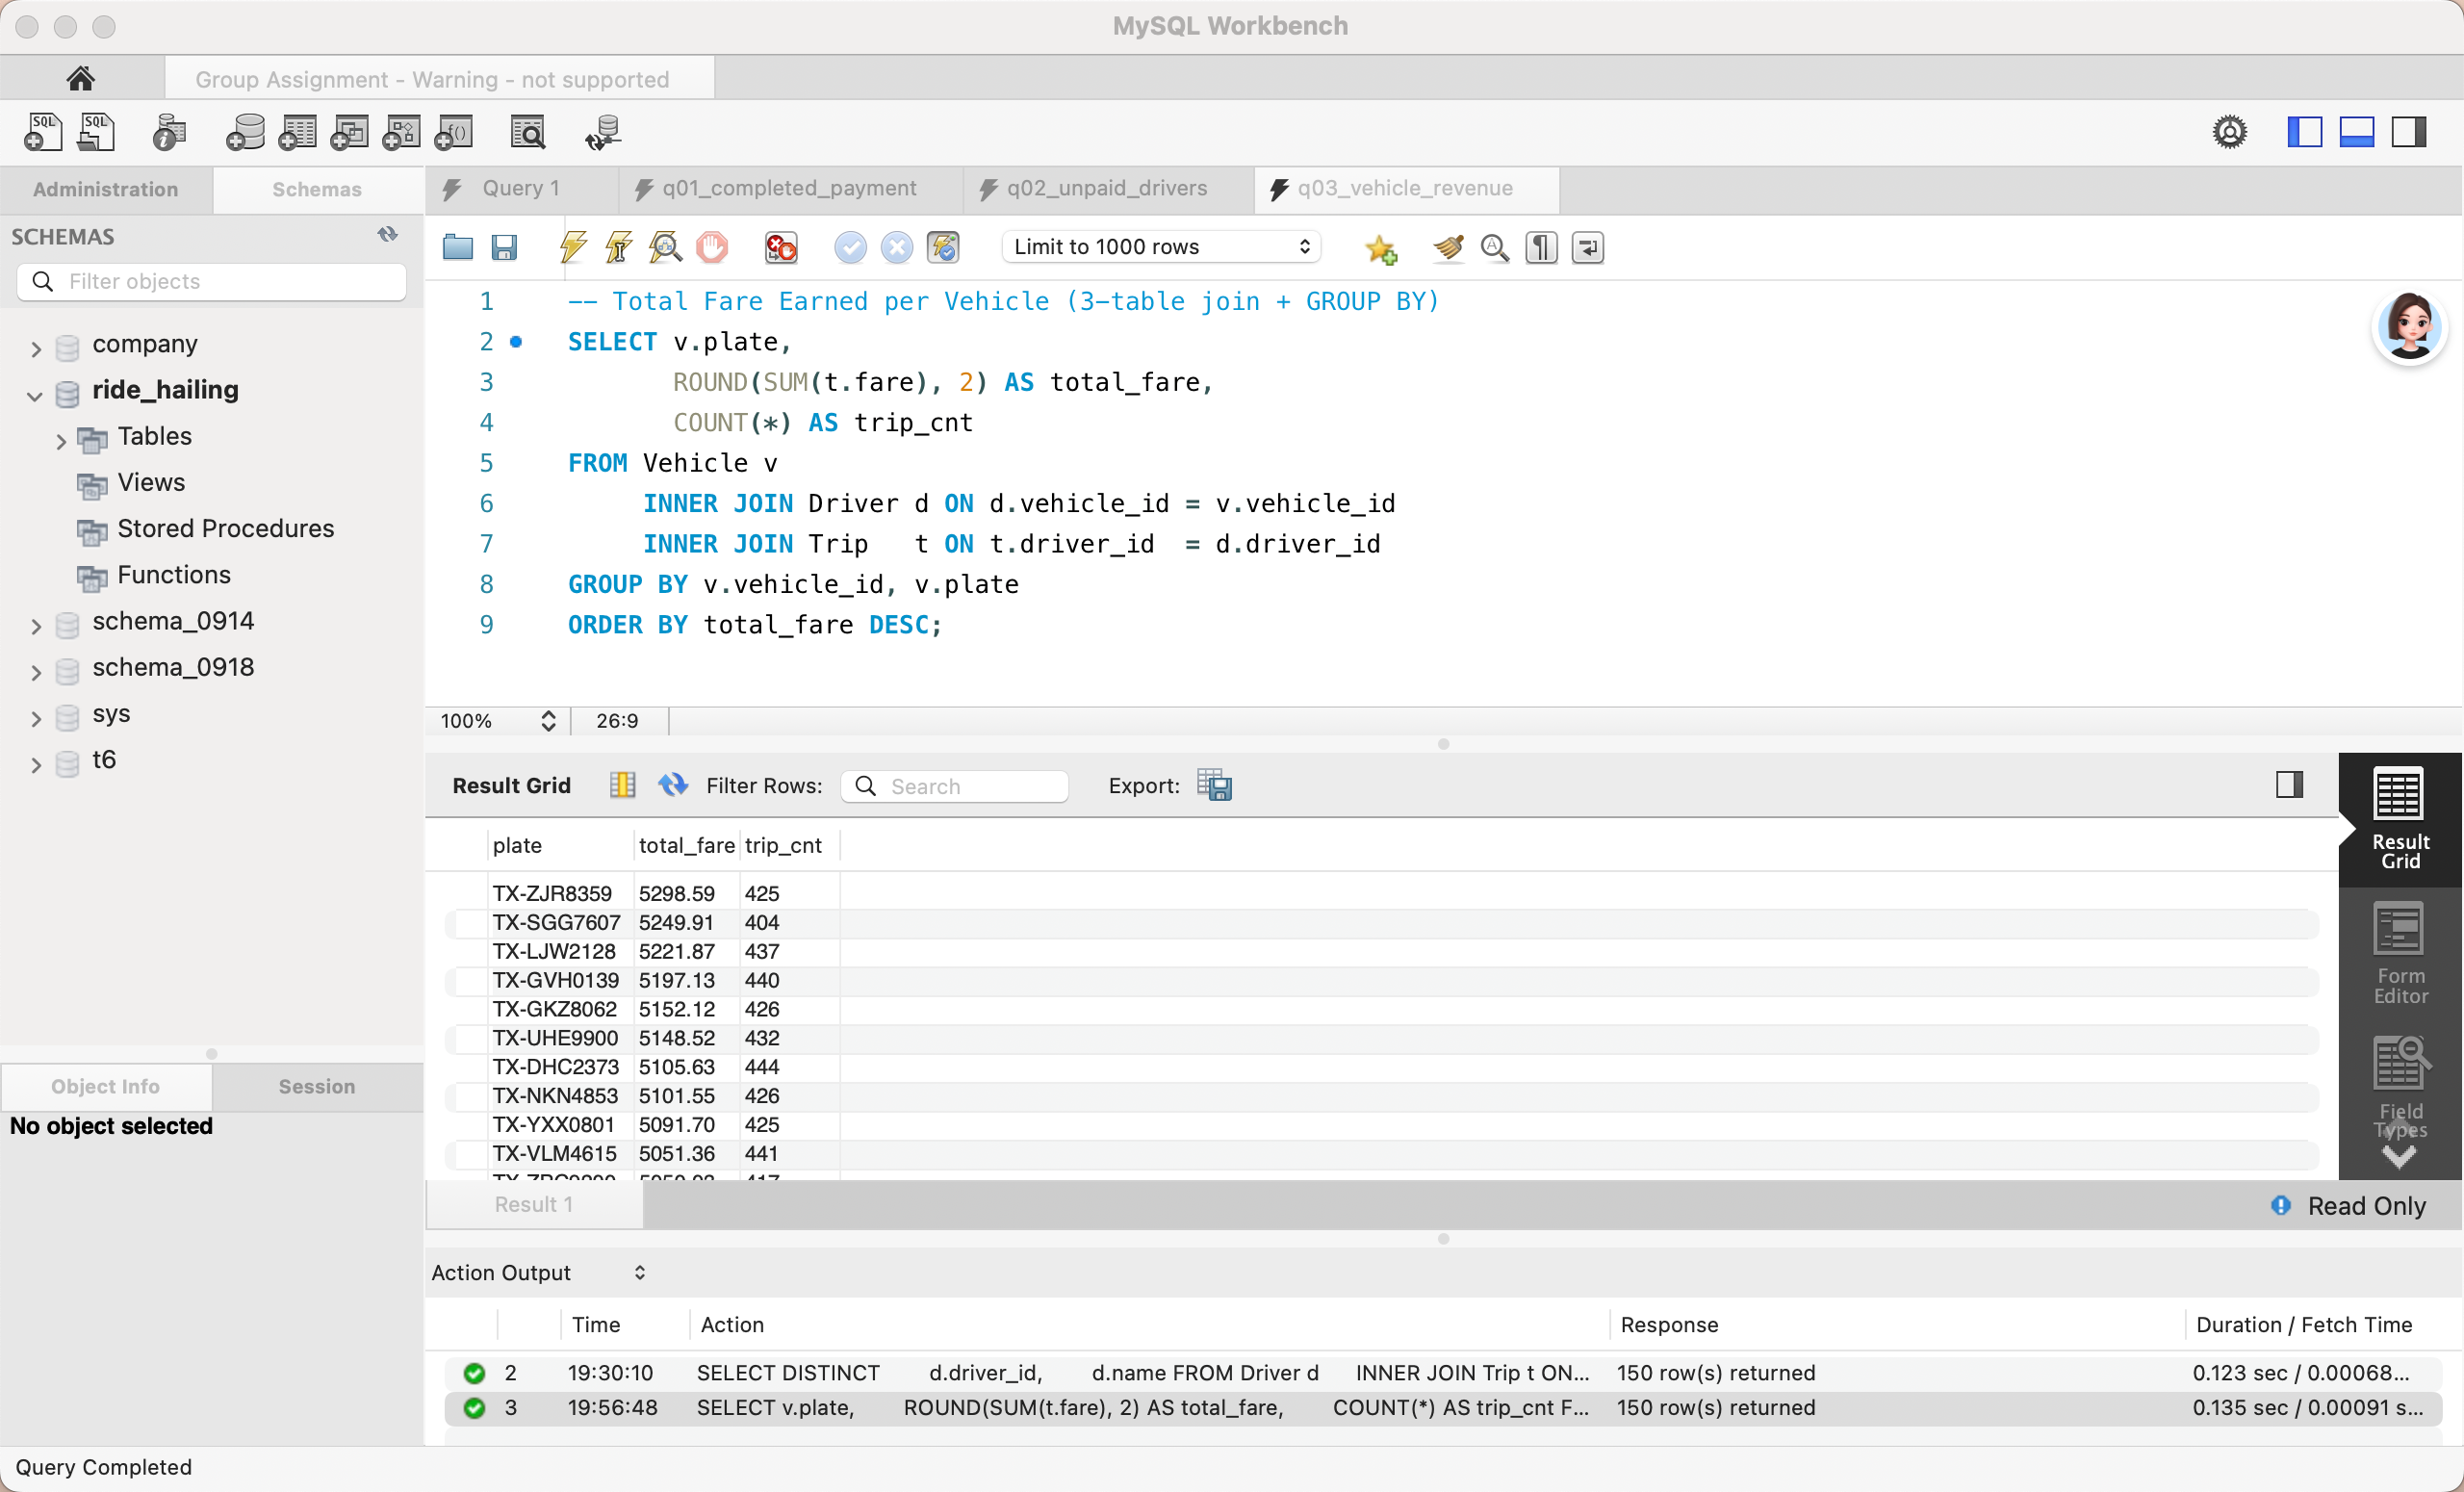
\includegraphics[width=\textwidth]{q03_vehicle_revenue_1029.png}
\caption{Q3: total fare per vehicle, 150-vehicle fleet.}
\end{figure}

\begin{figure}[ht]\centering
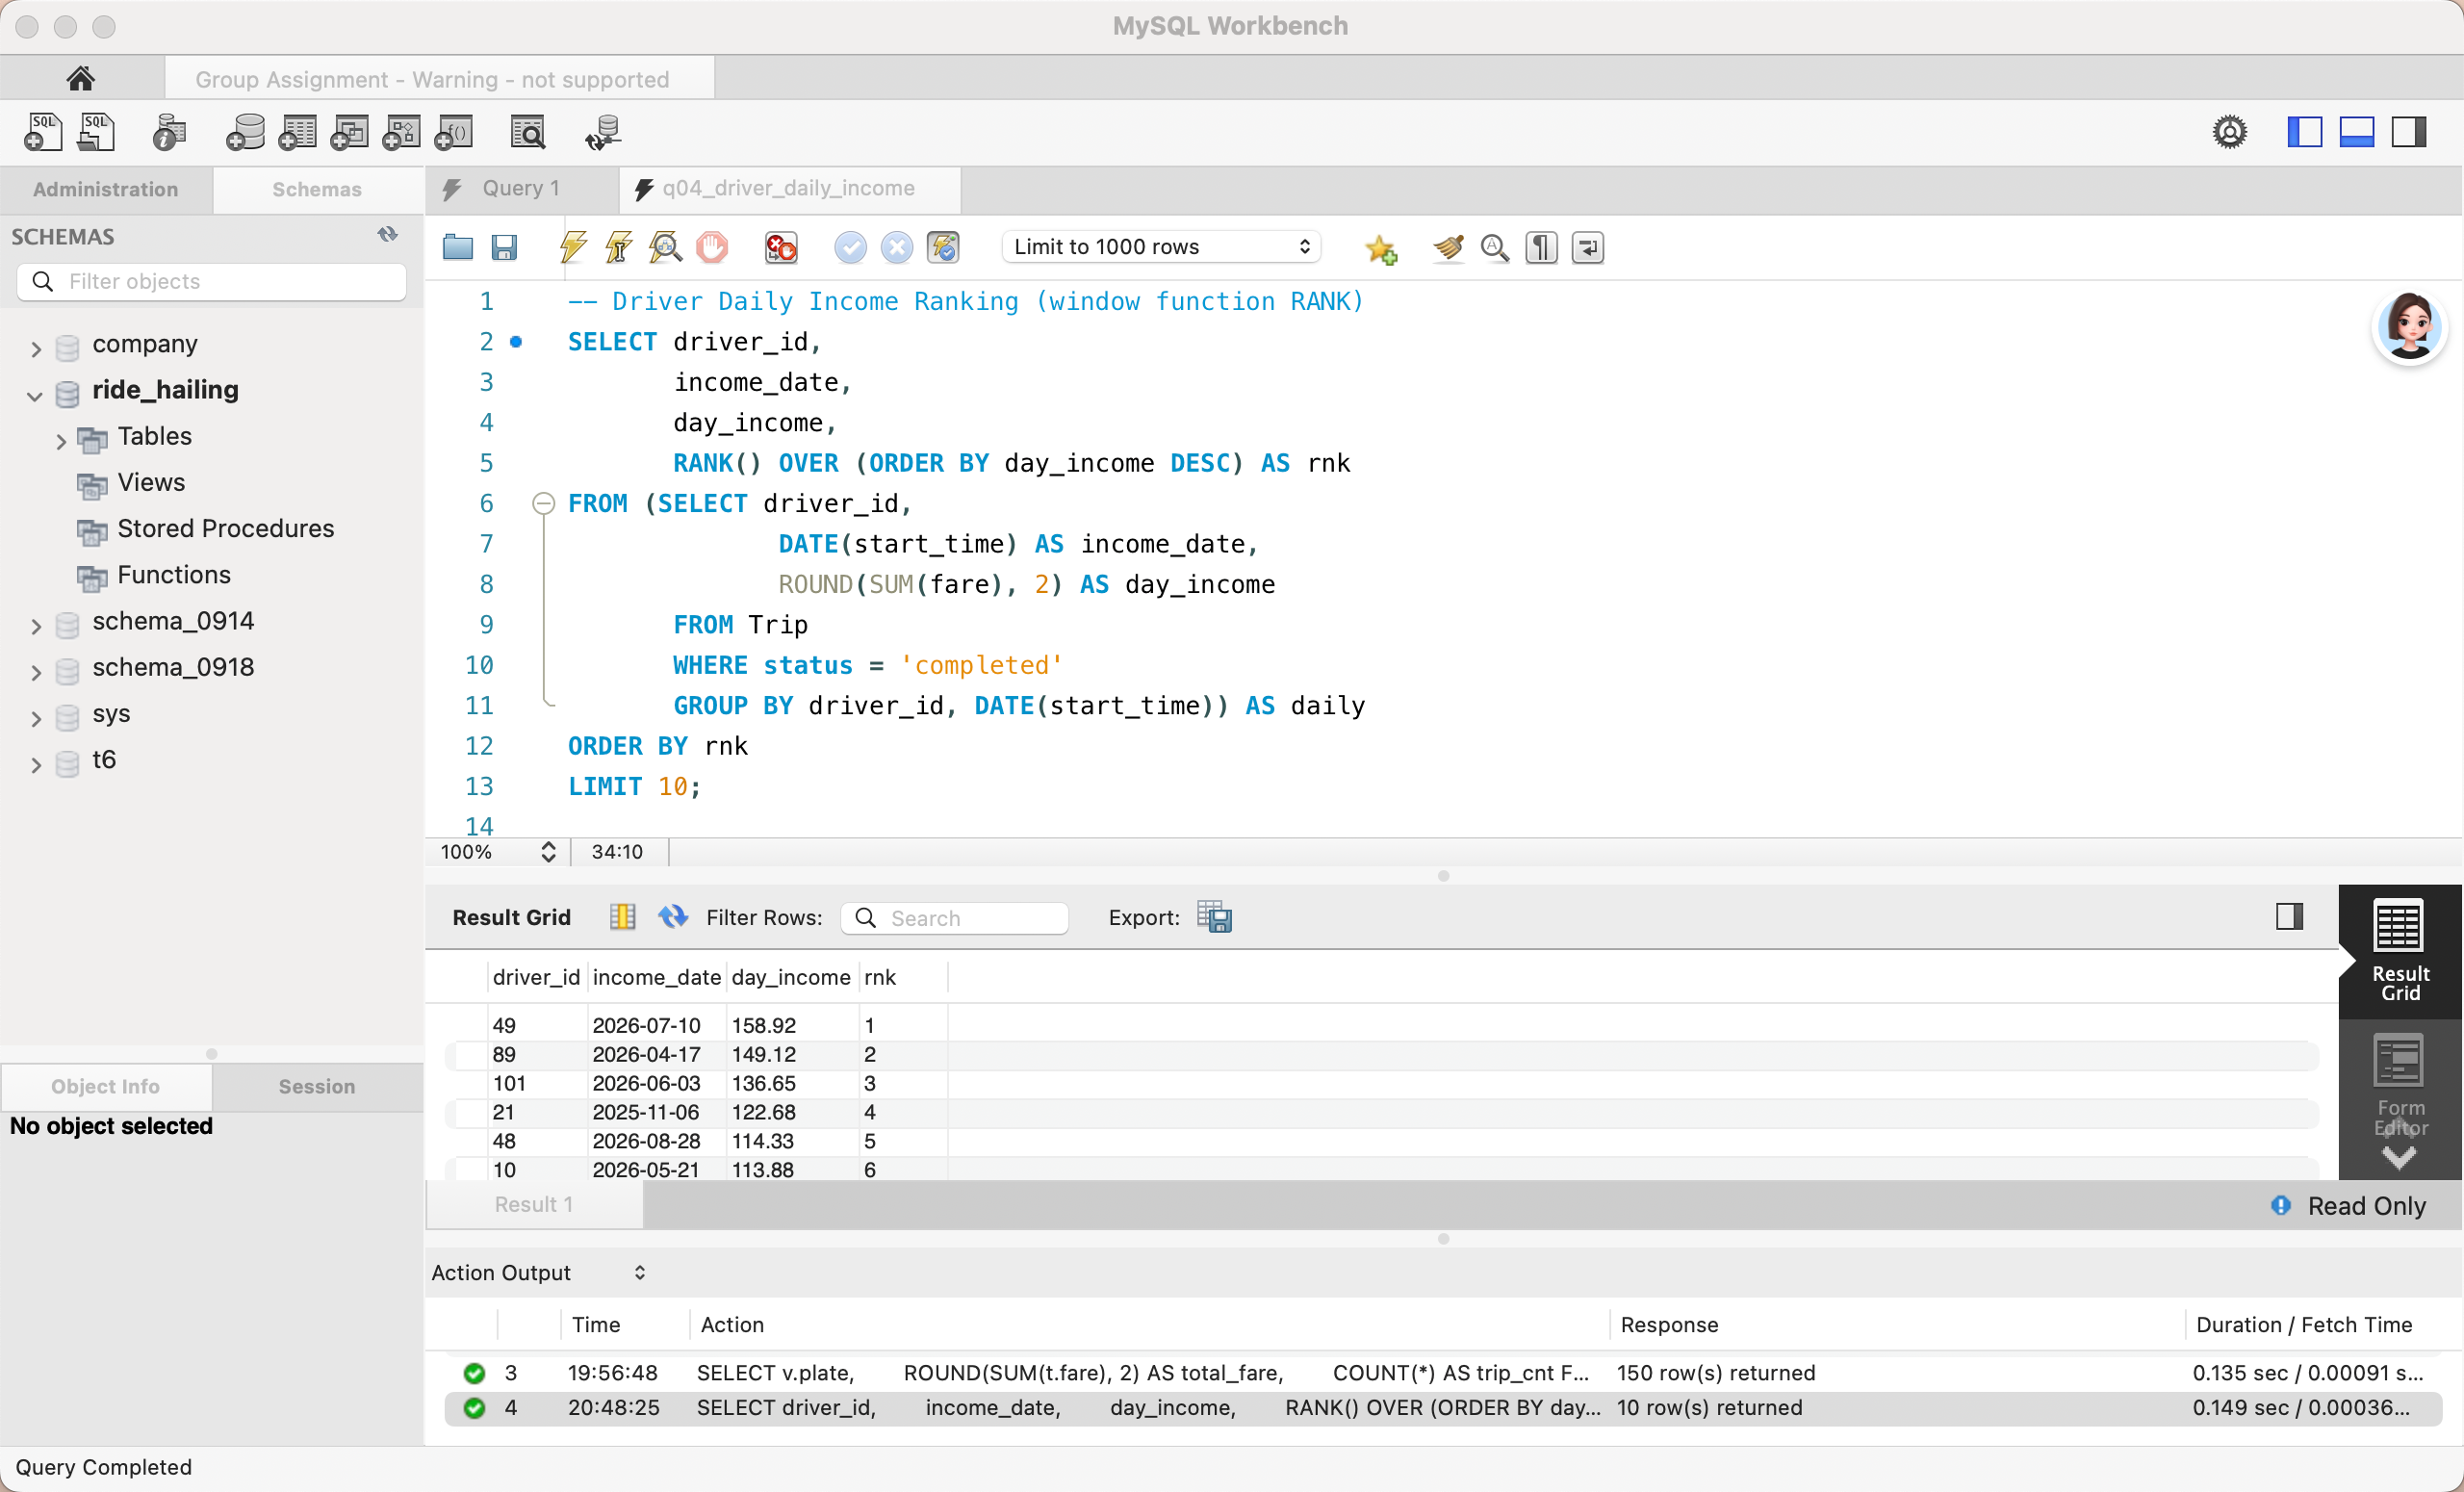
\includegraphics[width=\textwidth]{q04_driver_daily_income_1029.png}
\caption{Q4: driver daily income ranking, top-10 driver-days.}
\end{figure}

\begin{figure}[ht]\centering
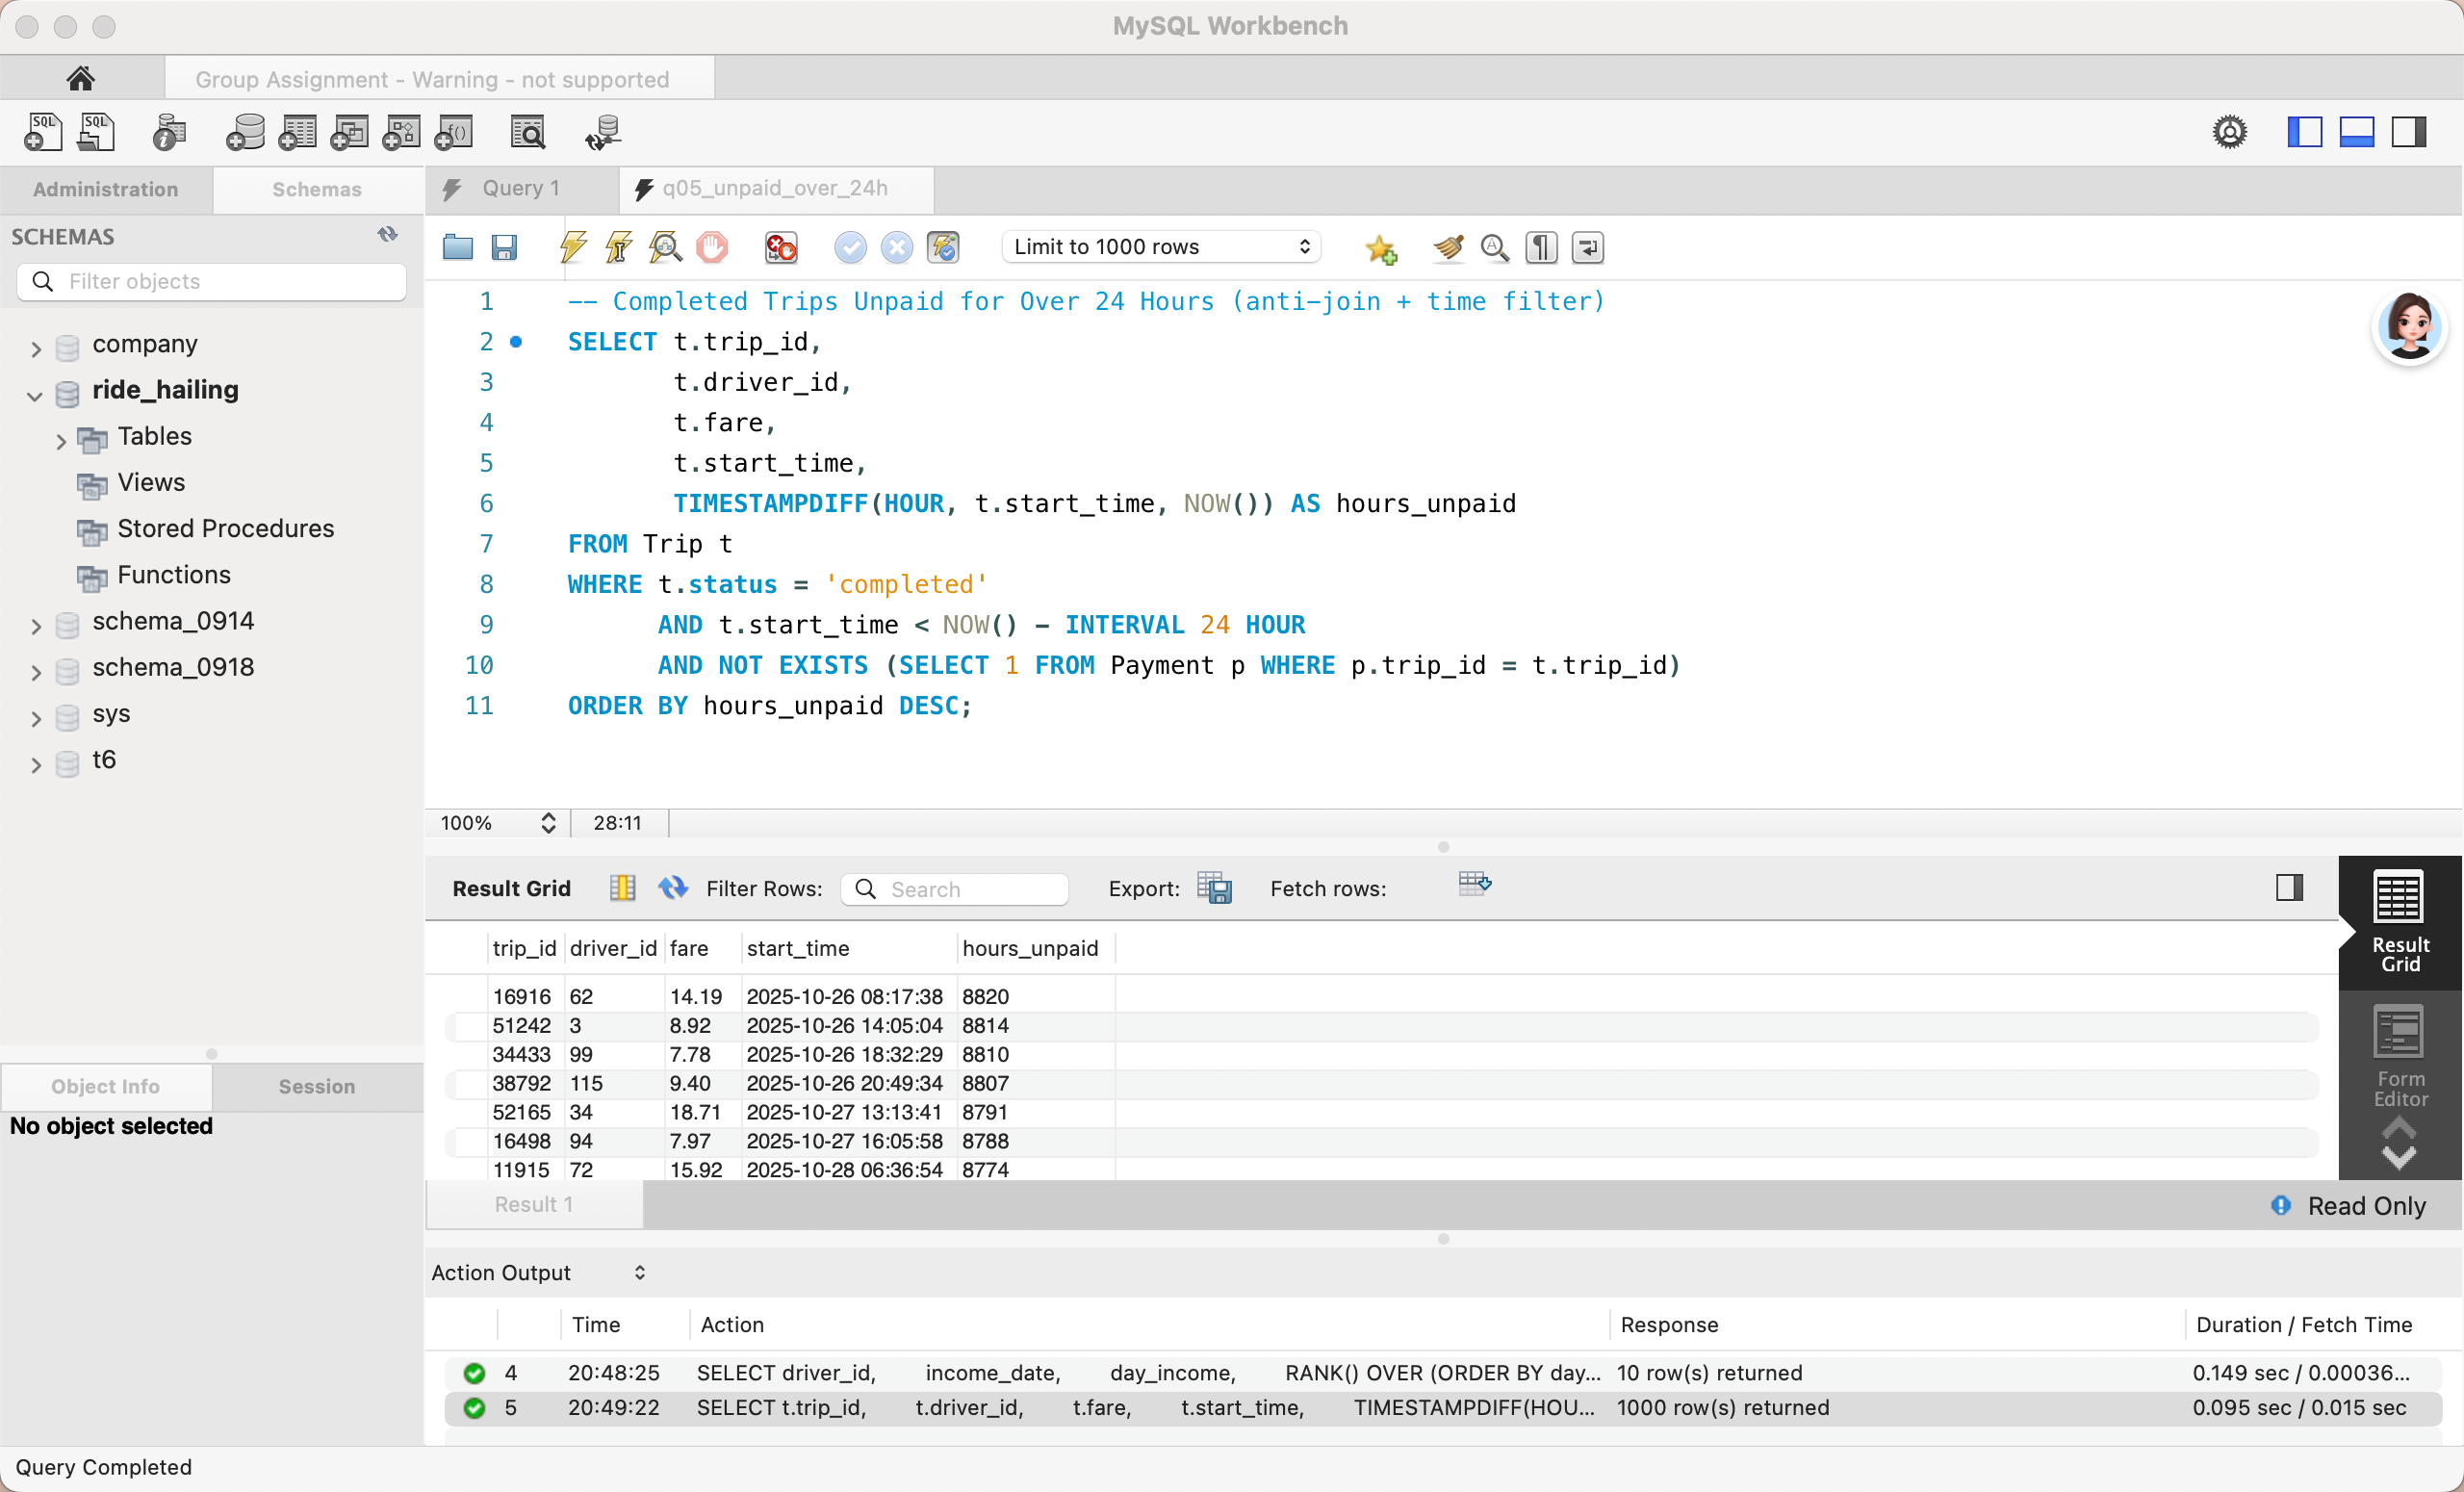
\includegraphics[width=\textwidth]{q05_unpaid_over_24h_1029.png}
\caption{Q5: completed and unpaid beyond 24 hours (first 1{,}000 of 1{,}442 rows).}
\end{figure}

\begin{figure}[ht]\centering
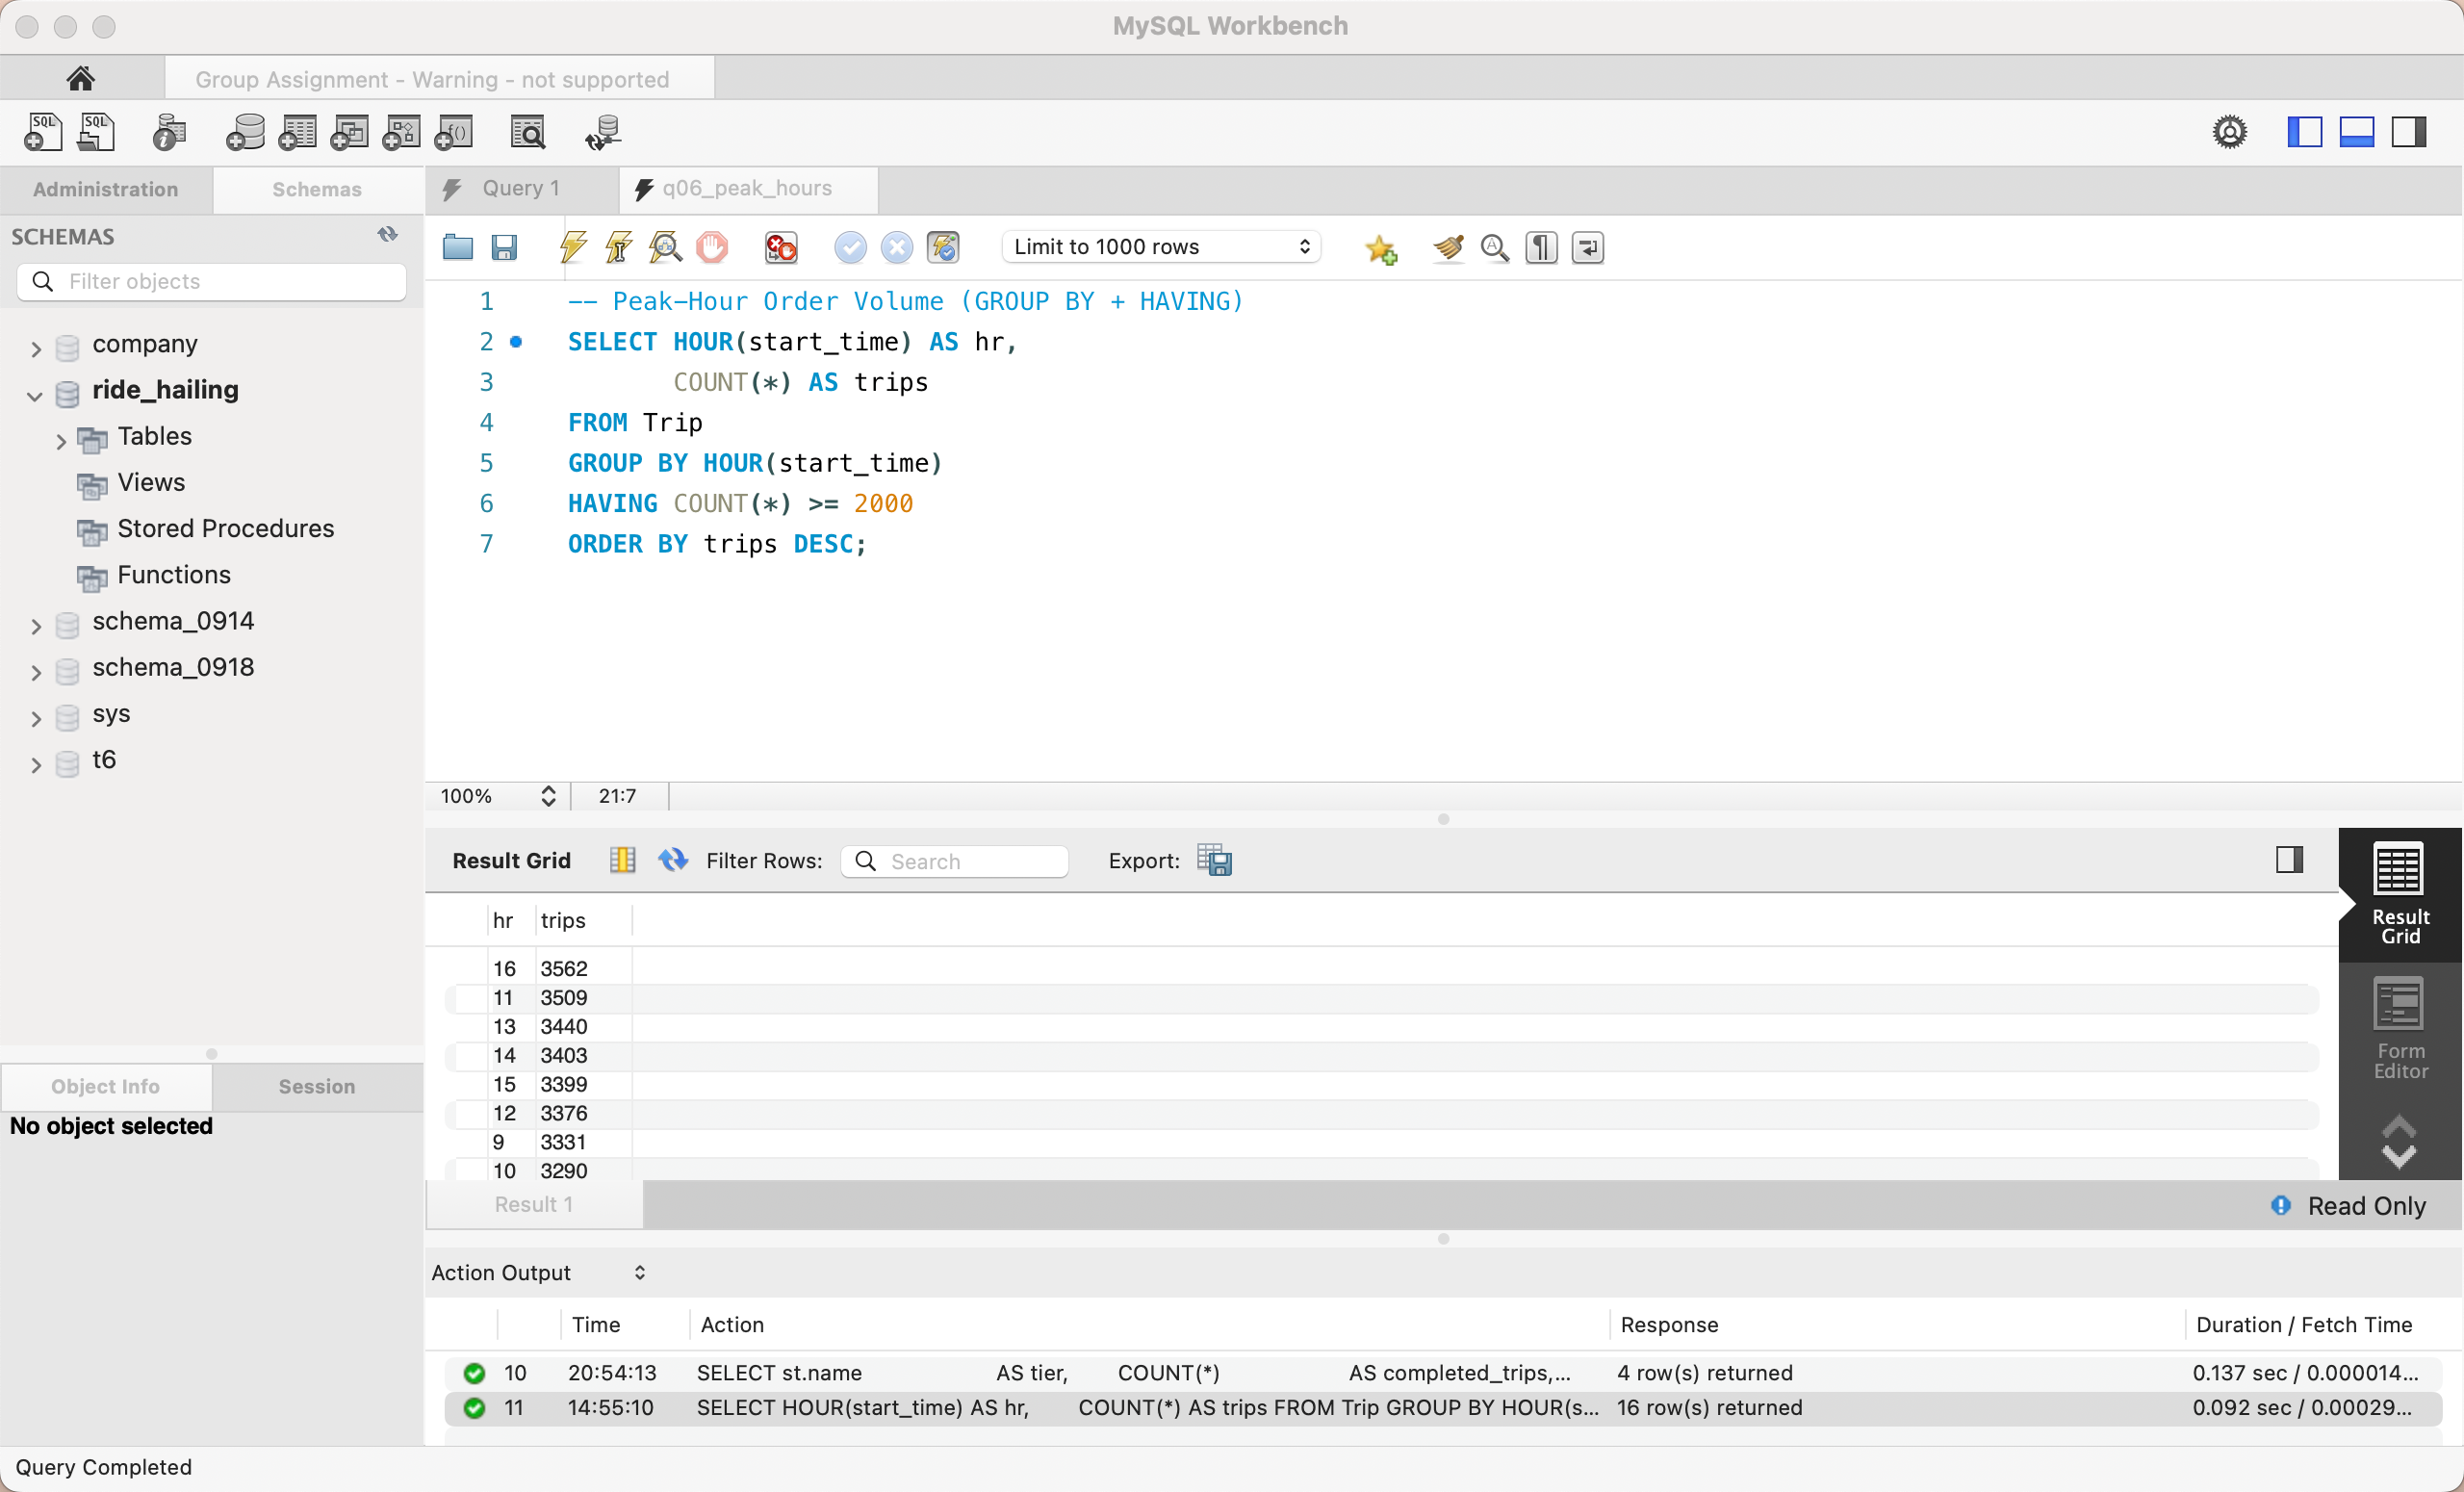
\includegraphics[width=\textwidth]{q06_peak_hours_1029.png}
\caption{Q6: peak-hour volume, 14 hours above the 2{,}000-trip threshold.}
\end{figure}

\begin{figure}[ht]\centering
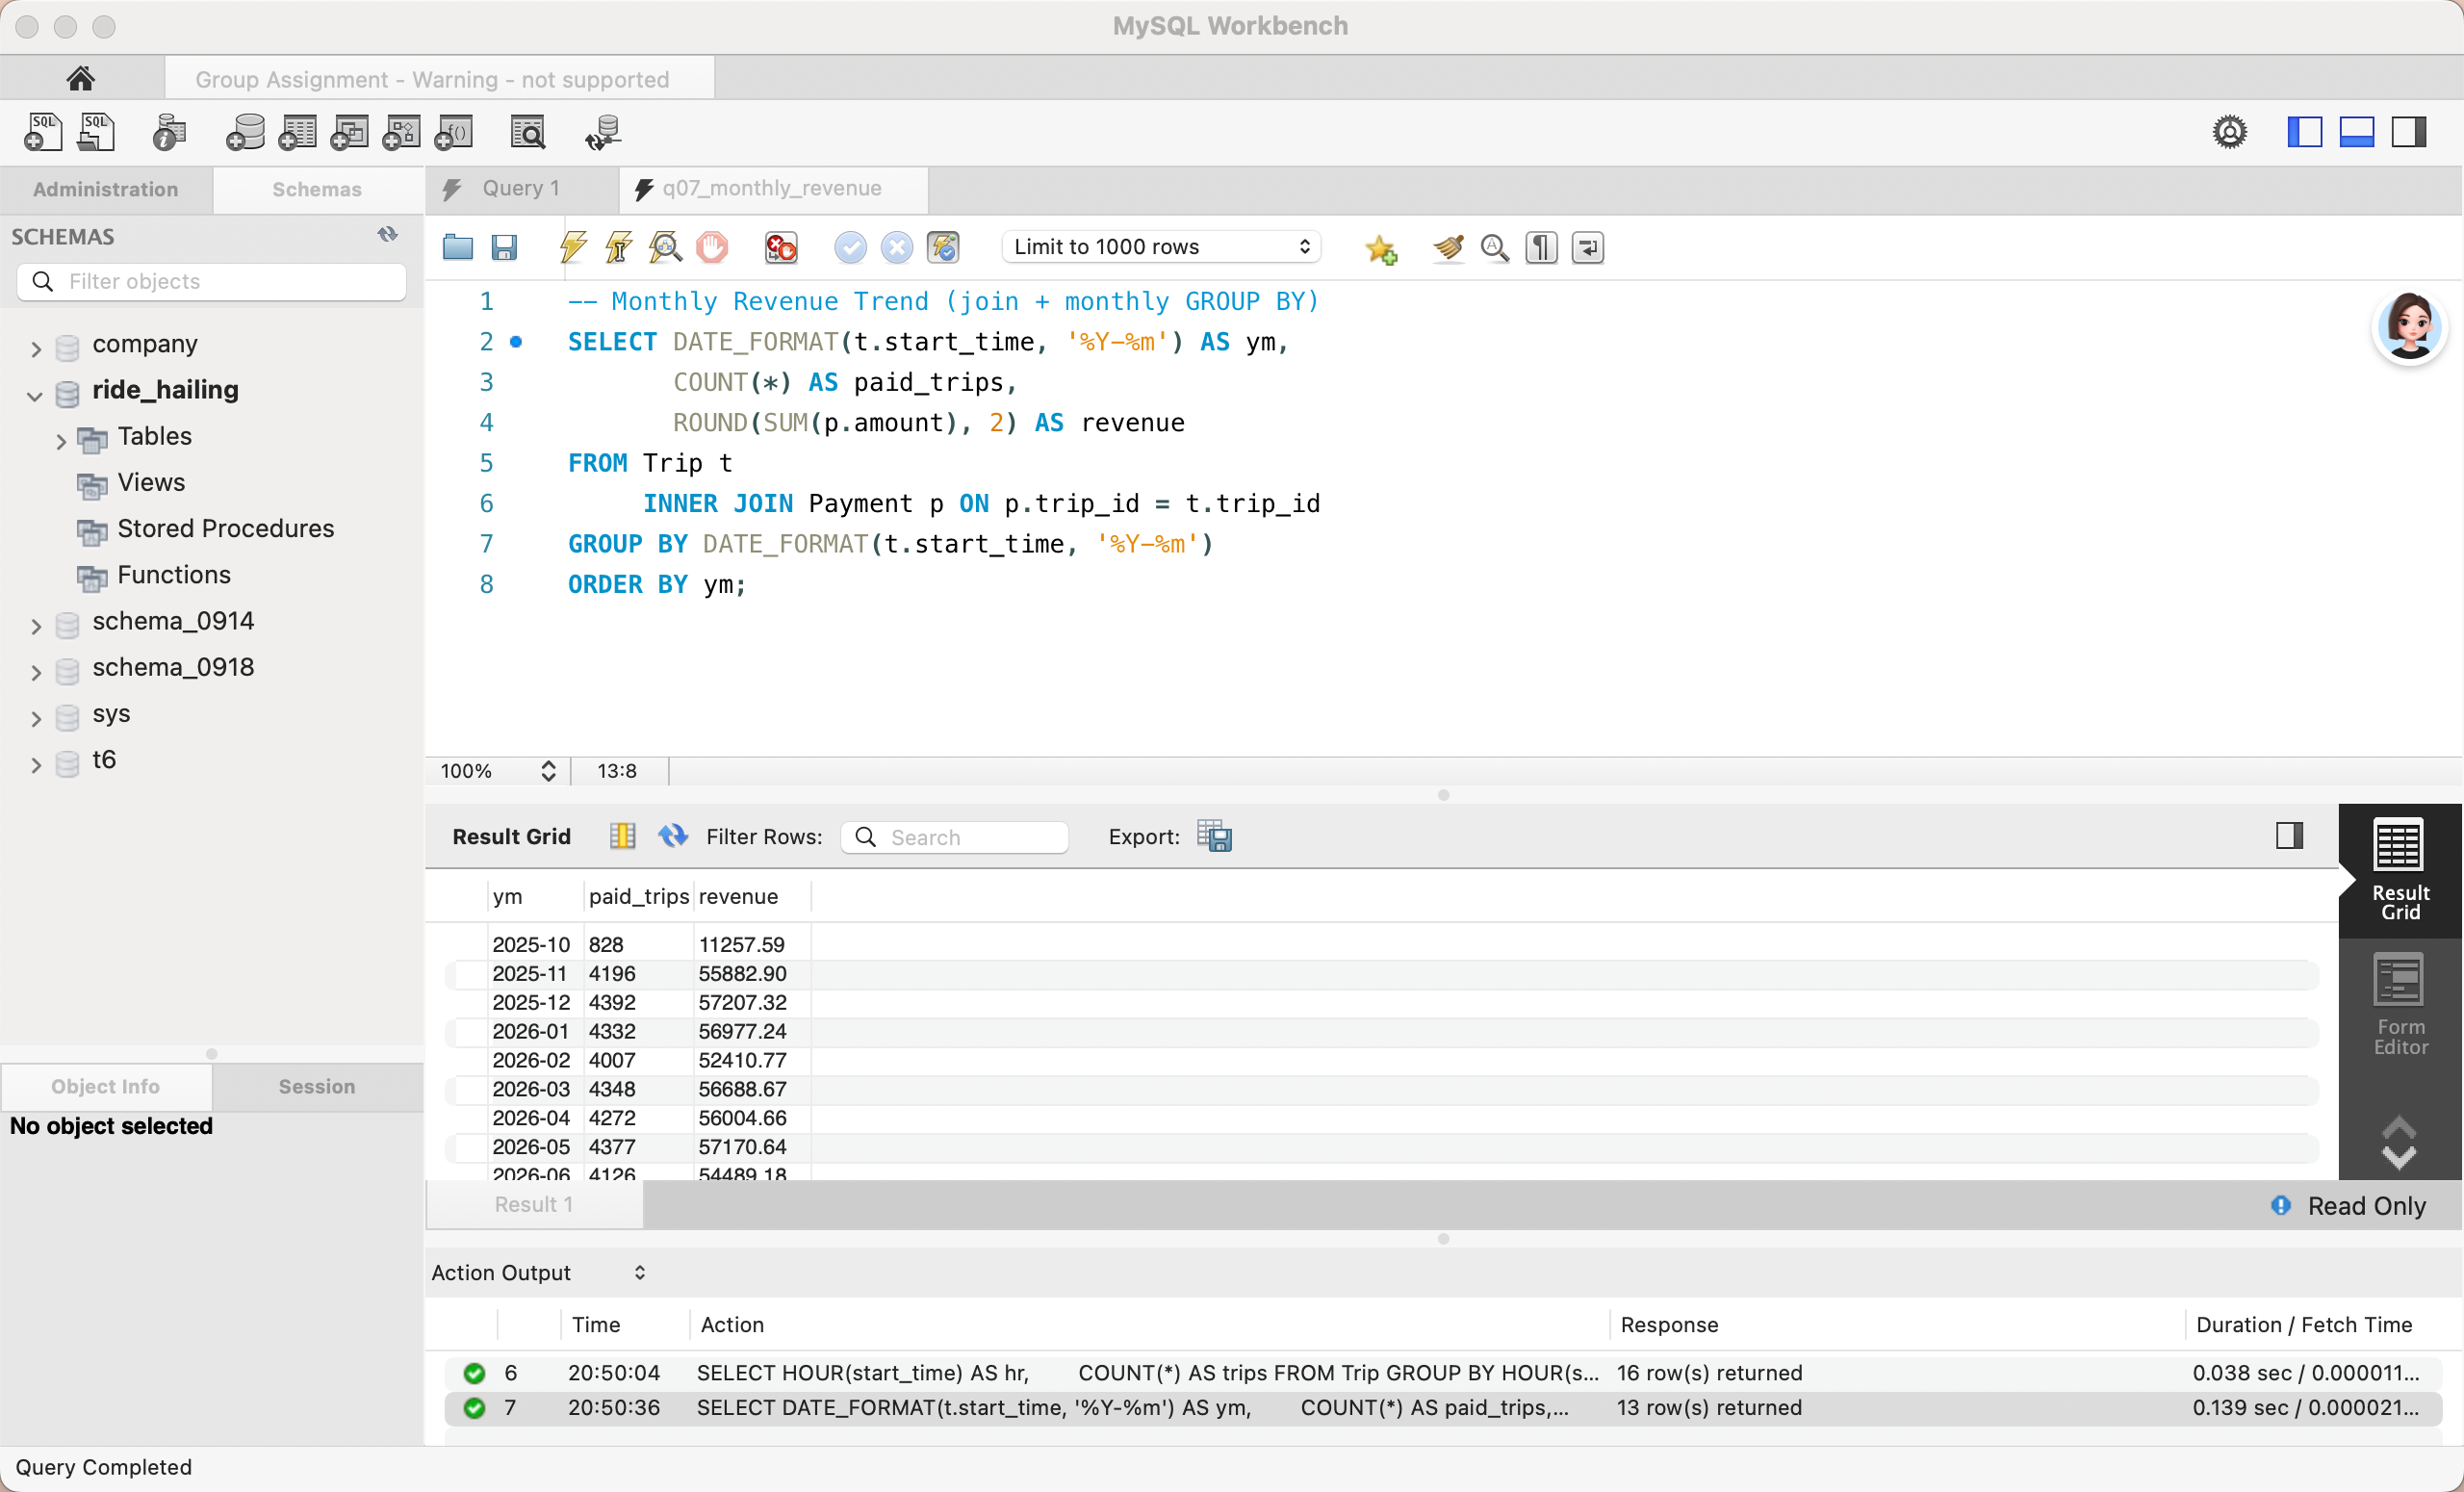
\includegraphics[width=\textwidth]{q07_monthly_revenue_1029.png}
\caption{Q7: monthly revenue over twelve months.}
\end{figure}

\begin{figure}[ht]\centering
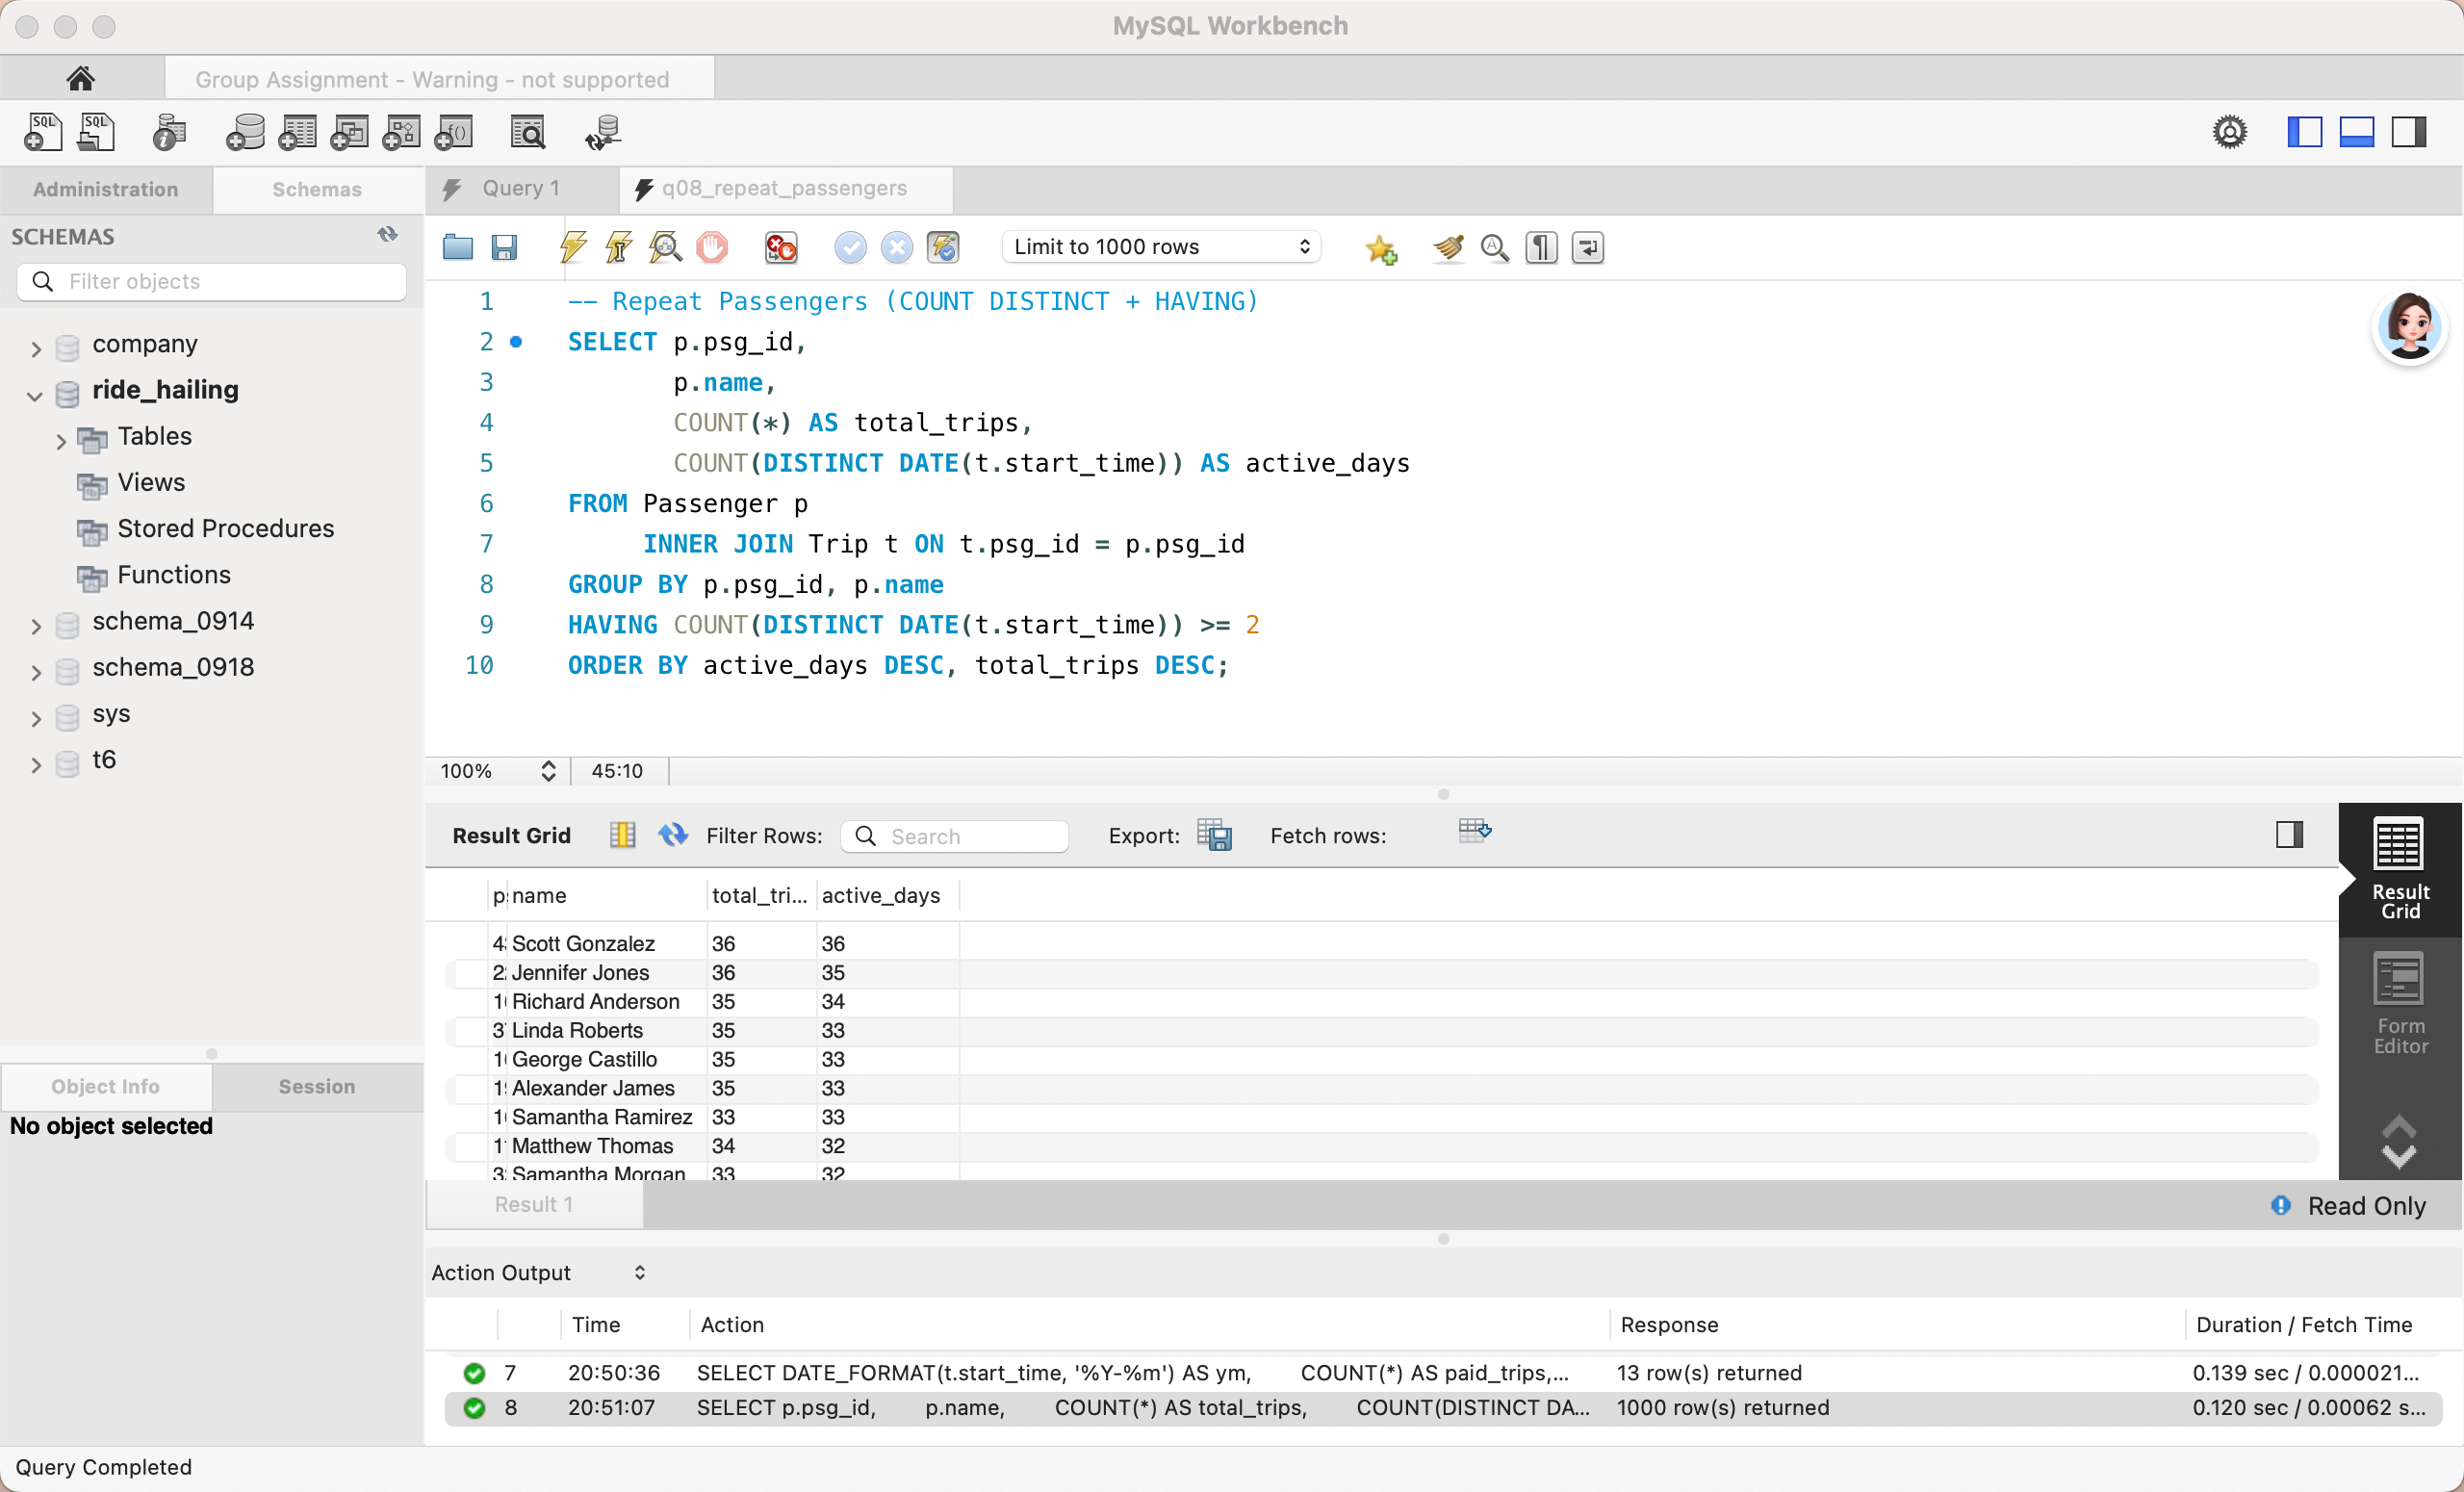
\includegraphics[width=\textwidth]{q08_repeat_passengers_1029.png}
\caption{Q8: repeat passengers (first 1{,}000 rows).}
\end{figure}
